\documentclass{beamer}
\usepackage{preamble_beamer}


\title[Введение]{Лекция 0. Intro} % The short title appears at the bottom of every slide, the full title is only on the title page


\begin{document}

\begin{frame}
\titlepage 
\end{frame}
\begin{frame}
\frametitle{О курсе} 
Преподаватели:
\begin{itemize} 
    \item Геннадий Пифтанкин -- мехмат МГУ, РЭШ, к.ф.м.н., Моделирование фин. рынков, Блок Риски, Сбер. 
    \item Александр Долматов -- физфак МГУ, РЭШ, Моделирование фин. рынков, Блок Риски, Сбер. 
\end{itemize}
\end{frame}

\begin{frame}{План курса}

\textbf{Теоретическая часть}
\begin{itemize}
    \item Случайные процессы в дискретном времени
    \item Случайные процессы в непрерывном времени: введение в стохастический анализ
    \item Стохастические дифференциальные уравнения
    \item Модель Блэка-Шоулза. Фундаментальные теоремы     
    \item Модели локальной и стохастической волатильности
\end{itemize}

\textbf{Численные методы}
\begin{itemize}
    \item Методы на основе деревьев и УРЧП
    \item Методы MC и American MC
    \item Численные методы для модели Хестона
    \item Численные методы для модели локальной волатильности
    \item* RL в финансах
    \item \href{https://github.com/dolmatovas/quant_finance_hse/tree/main/projects}{Проекты} 
\end{itemize}
\end{frame}

\begin{frame}{Историческое развитие моделей}
\footnotesize
\begin{itemize}
\item \textbf{Модель Башелье} (1900). Случайное блуждание цен активов \\ 
\begin{scriptsize}{\textit{Bachelier L. Théorie de la spéculation (1900)}}\end{scriptsize}

\item \textbf{Аксиоматика вероятностей} (1933). Существование винеровского процесса \\
\begin{scriptsize}{\textit{Колмогоров А.Н. Основные понятия теории вероятностей (1933)}}\end{scriptsize}

\item \textbf{Стохастическое исчисление} (1944). Интеграл Ито \\
\begin{scriptsize}{\textit{Itô K. Stochastic Integral (1944)}}\end{scriptsize}

\item \textbf{Модель Блэка-Шоулза} (1973). Прайсинг через репликацию \\
\begin{scriptsize}{\textit{Black F., Scholes M. The Pricing of Options (1973)}}\end{scriptsize}

\item \textbf{Риск-нейтральный прайсинг} (1976-1981). Фундаментальные теоремы финансов\\
\begin{scriptsize}{\textit{Harrison J.M., Kreps D.M. (1979); Harrison J.M., Pliska S.R. (1981)}}\end{scriptsize}
\end{itemize}
\end{frame}

\begin{frame}{Историческое развитие моделей}
\footnotesize
\begin{itemize}


\item \textbf{Модели стохастической волатильности} (1993). Отказ от постоянной волатильности, тяжелые хвосты. \\
Модель Хестона \scriptsize{\textit{Heston S.L. A Closed-Form Solution (1993)}}
\\Формула Дюпира 
\begin{scriptsize}{\textit{Dupire B. Pricing with a Smile (1994)}}\end{scriptsize}

\item \textbf{Кредитный риск} (2009-2010). xVA. Реакция на кризиз 2008 года \\
\begin{scriptsize}{\textit{BIS Basel III Framework (2010); Pykhtin M., Zhu S. (2007)}}\end{scriptsize}

\item \textbf{Микроструктура рынка} (1985-2018). Модель Кайла. Deep Hedging \\
\begin{scriptsize}{\textit{Kyle A.S. Continuous Auctions (1985); Bühler H. et al. (2019)}}\end{scriptsize}

\item \textbf{Децентрализованные финансы} (2008-). Блокчейн, смарт-контракты, Automated Market Makers\\
\begin{scriptsize}{\textit{Nakamoto S. Bitcoin Whitepaper (2008)}}\end{scriptsize} \\
\begin{scriptsize}{\textit{Buterin V. Ethereum Whitepaper (2014)}}\end{scriptsize} \\
\begin{scriptsize}{\textit{Adams H. Uniswap v3 Core (2021)}}\end{scriptsize}

\item \textbf{Машинное обучение} (2010-) Алгоритмический трейдинг, прогнозирование 
\begin{scriptsize}{\textit{Lo A.W. Adaptive Markets (2017)}}\end{scriptsize}
\\ Генеративные модели
\begin{scriptsize} \textit{Hans Buehler, Generating Financial Markets With Signatures (2021)} \end{scriptsize}
\end{itemize}
\end{frame}

\begin{frame}{Эволюция методов прайсинга}
    \begin{center}
        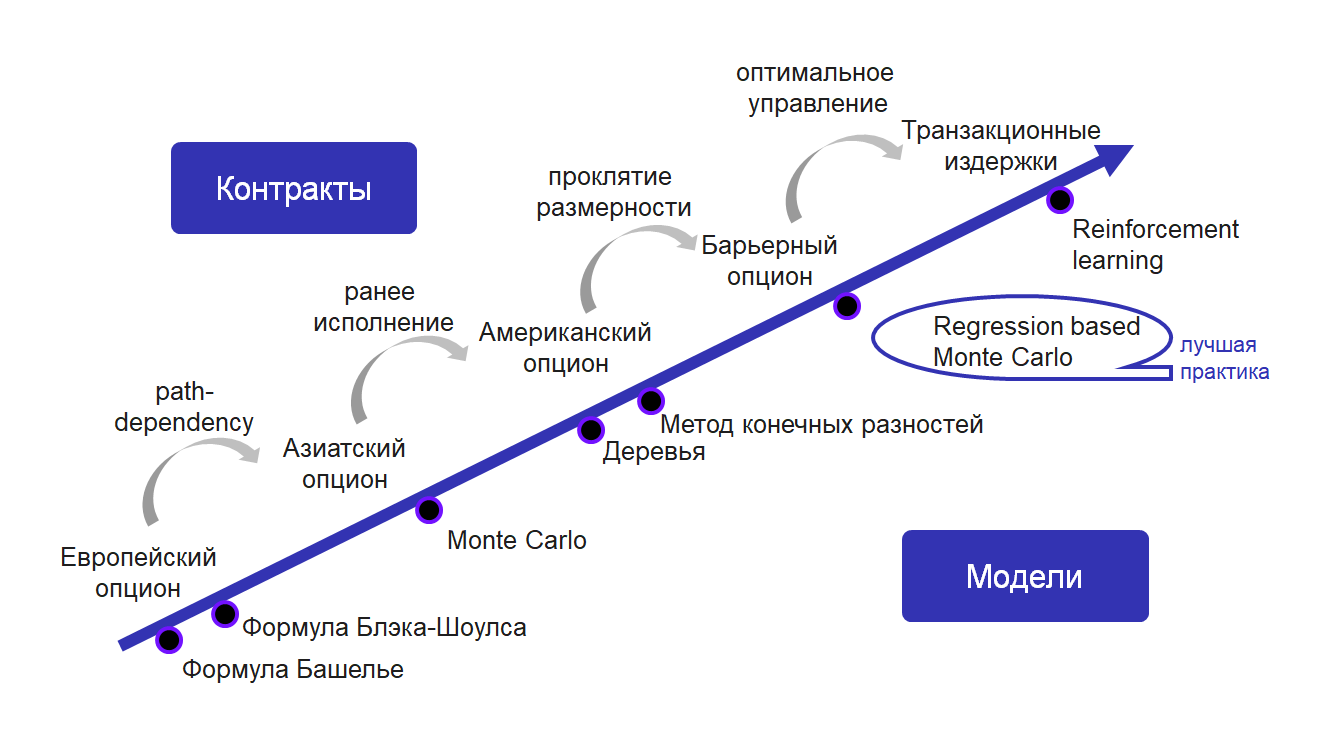
\includegraphics[width=1.0\textwidth]{0_figs/стрелочка.png}
    \end{center}
\end{frame}



\end{document}